\subsection{OpenMP of the Jacobi Method}
The Jacobi method updates a new matrix from the values of an old one, and it is thus easily parallelizable. The program is paralellized using orphaning in openMP. The \texttt{\#pragma omp parallel} is inside the while loop described above. That has the obvious disadvantage that the worker team will be created and destroyed with each iteration, creating a lot of overhead that will reduce performance. The speed up of the the initial implementation is seen in figure \ref{fig:omp_scale1}. \begin{huge}
DESCRIBE FIGURE \ref{fig:omp_scale1} HERE
\end{huge}

\begin{figure}
\centering
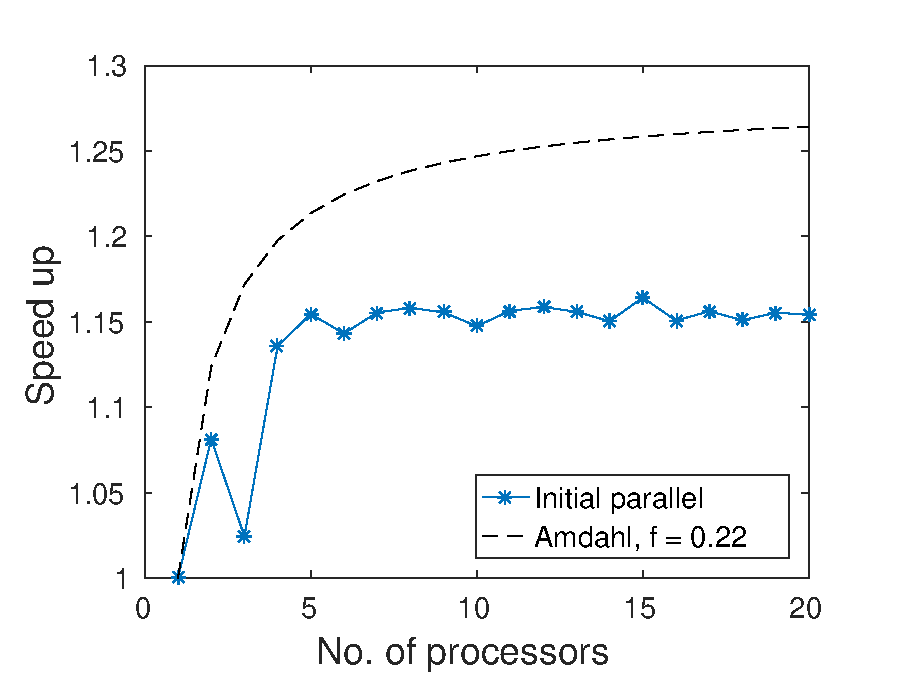
\includegraphics[width = 0.8\textwidth]{fig/speedup_omp.eps}
\caption{Scaling of the first parallelized version.}
\label{fig:omp_scale1}
\end{figure}

To investigate the lack of speed up, the program is sent through the Sun Studio Performance Analyzer tool in sequential mode to see the fraction of time  spent in the parallelized region, to facilitate a comparison with Amdahl's law. 